\section{\RU{Подсчет выставленных бит}\EN{Counting bits set to 1}}

\RU{Вот этот несложный пример иллюстрирует функцию, считающую количество бит-единиц во входном значении.}
\EN{Here is a simple example of a function that calculates the number of bits set in the input value.}

\RU{Эта операция также называется}\EN{This operation is also called} ``population count''
\footnote{\RU{современные x86-процессоры (поддерживающие SSE4) даже имеют инструкцию POPCNT для этого}
\EN{modern x86 CPUs (supporting SSE4) even have a POPCNT instruction for it}}.

\lstinputlisting{patterns/14_bitfields/4_popcnt/shifts.c}

\RU{В этом цикле, счетчик итераций $i$ считает от $0$ до $31$, а $1 \ll i$ будет от $1$ до \TT{0x80000000}. 
Описывая это словами, можно сказать, 
\IT{сдвинуть единицу на $n$ бит влево}.
Т.е., в некотором смысле, выражение $1 \ll i$ последовательно выдаст все возможные позиции бит в 32-битном числе. 
Освободившийся бит справа всегда обнуляется.}
\EN{In this loop, the iteration count value $i$ is counting from $0$ to $31$, so the $1 \ll i$ statement will be counting 
from $1$ to \TT{0x80000000}.
Describing this operation in natural language, we would say \IT{shift $1$ by n bits left}.
In other words, $1 \ll i$ statement will consequently produce all possible bit positions in a 32-bit number.
The freed bit at right is always cleared.}

\RU{Вот таблица всех возможных значений}\EN{Here is a table of all possible} $1 \ll i$ 
\RU{для}\EN{for} $i=0 \ldots 31$:

\begin{center}
\begin{tabular}{ | l | l | l | l | }
\hline
\cellcolor{blue!25} \RU{Выражение в }\CCpp\EN{ expression} & 
\cellcolor{blue!25} \RU{Степень двойки}\EN{Power of two} & 
\cellcolor{blue!25} \RU{Десятичная форма}\EN{Decimal form} & 
\cellcolor{blue!25} \RU{Шестнадцатеричная форма}\EN{Hexadecimal form} \\
\hline
$1 \ll 0$ & 1 & 1 & 1 \\
\hline
$1 \ll 1$ & $2^{1}$ & 2 & 2 \\
\hline
$1 \ll 2$ & $2^{2}$ & 4 & 4 \\
\hline
$1 \ll 3$ & $2^{3}$ & 8 & 8 \\
\hline
$1 \ll 4$ & $2^{4}$ & 16 & 0x10 \\
\hline
$1 \ll 5$ & $2^{5}$ & 32 & 0x20 \\
\hline
$1 \ll 6$ & $2^{6}$ & 64 & 0x40 \\
\hline
$1 \ll 7$ & $2^{7}$ & 128 & 0x80 \\
\hline
$1 \ll 8$ & $2^{8}$ & 256 & 0x100 \\
\hline
$1 \ll 9$ & $2^{9}$ & 512 & 0x200 \\
\hline
$1 \ll 10$ & $2^{10}$ & 1024 & 0x400 \\
\hline
$1 \ll 11$ & $2^{11}$ & 2048 & 0x800 \\
\hline
$1 \ll 12$ & $2^{12}$ & 4096 & 0x1000 \\
\hline
$1 \ll 13$ & $2^{13}$ & 8192 & 0x2000 \\
\hline
$1 \ll 14$ & $2^{14}$ & 16384 & 0x4000 \\
\hline
$1 \ll 15$ & $2^{15}$ & 32768 & 0x8000 \\
\hline
$1 \ll 16$ & $2^{16}$ & 65536 & 0x10000 \\
\hline
$1 \ll 17$ & $2^{17}$ & 131072 & 0x20000 \\
\hline
$1 \ll 18$ & $2^{18}$ & 262144 & 0x40000 \\
\hline
$1 \ll 19$ & $2^{19}$ & 524288 & 0x80000 \\
\hline
$1 \ll 20$ & $2^{20}$ & 1048576 & 0x100000 \\
\hline
$1 \ll 21$ & $2^{21}$ & 2097152 & 0x200000 \\
\hline
$1 \ll 22$ & $2^{22}$ & 4194304 & 0x400000 \\
\hline
$1 \ll 23$ & $2^{23}$ & 8388608 & 0x800000 \\
\hline
$1 \ll 24$ & $2^{24}$ & 16777216 & 0x1000000 \\
\hline
$1 \ll 25$ & $2^{25}$ & 33554432 & 0x2000000 \\
\hline
$1 \ll 26$ & $2^{26}$ & 67108864 & 0x4000000 \\
\hline
$1 \ll 27$ & $2^{27}$ & 134217728 & 0x8000000 \\
\hline
$1 \ll 28$ & $2^{28}$ & 268435456 & 0x10000000 \\
\hline
$1 \ll 29$ & $2^{29}$ & 536870912 & 0x20000000 \\
\hline
$1 \ll 30$ & $2^{30}$ & 1073741824 & 0x40000000 \\
\hline
$1 \ll 31$ & $2^{31}$ & 2147483648 & 0x80000000 \\
\hline
\end{tabular}
\end{center}

\RU{Это числа-константы (битовые маски), которые крайне часто попадаются в практике reverse engineer-а, 
и их нужно уметь распознавать.}
\EN{These constant numbers (bit masks) very often appear in code and a practicing reverse engineer 
has to be able to spot them quickly.}
\RU{Числа в десятичном виде заучивать, пожалуй, незачем, а числа в шестнадцатеричном
виде итак легко запомнить.}
\EN{You probably haven't to memorize the decimal numbers, but the hexadecimal ones are very easy to remember.}

\RU{Эти константы очень часто используются для определения отдельных бит как флагов.}
\EN{These constants are very often used for mapping flags to specific bits.}
\RU{Например, это из файла}\EN{For example, here is excerpt from} \TT{ssl\_private.h} \RU{из исходников}
\EN{from} Apache 2.4.6\EN{ source code}:

\begin{lstlisting}
/**
 * Define the SSL options
 */
#define SSL_OPT_NONE           (0)
#define SSL_OPT_RELSET         (1<<0)
#define SSL_OPT_STDENVVARS     (1<<1)
#define SSL_OPT_EXPORTCERTDATA (1<<3)
#define SSL_OPT_FAKEBASICAUTH  (1<<4)
#define SSL_OPT_STRICTREQUIRE  (1<<5)
#define SSL_OPT_OPTRENEGOTIATE (1<<6)
#define SSL_OPT_LEGACYDNFORMAT (1<<7)
\end{lstlisting}

\RU{Вернемся назад к нашему примеру}\EN{Let's get back to our example}.

\RU{Макрос \TT{IS\_SET} проверяет наличие этого бита в $a$.}
\EN{The \TT{IS\_SET} macro checks bit presence in $a$.}

\index{x86!\Instructions!AND}
\RU{Макрос \TT{IS\_SET} на самом деле это операция логического И (\IT{AND}) 
и она возвращает $0$ если бита там нет, 
либо эту же битовую маску, если бит там есть. 
В \CCpp, конструкция \TT{if()} срабатывает, если выражение внутри её не ноль, пусть хоть $123456$, 
поэтому все будет работать.}
\EN{The \TT{IS\_SET} macro is in fact the logical AND operation (\IT{AND}) 
and it returns $0$ if the specific bit is absent there,
or the bit mask, if the bit is present.
\IT{The if()} operator in \CCpp triggers if the expression in it is not zero, it might be even $123456$, that is why
it always works correctly.}

% subsections
\subsection{x86}

\subsubsection{MSVC}

\RU{Компилируем}\EN{Let's compile} (MSVC 2010):

\lstinputlisting[caption=MSVC 2010]{patterns/14_bitfields/4_popcnt/shifts_MSVC.asm.\LANG}

\clearpage
\myparagraph{\olly}
\index{\olly}

\RU{Загрузим этот пример в}\EN{Let's load this example into} \olly. 
\RU{Входное значения для ф-ции пусть будет}\EN{Let's input value be} \TT{0x12345678}.\\
\\
\RU{Для}\EN{For} $i=1$, \RU{мы видим, как}\EN{we see how} $i$ \RU{загружается в}\EN{is loaded into} \ECX: 

\begin{figure}[H]
\centering
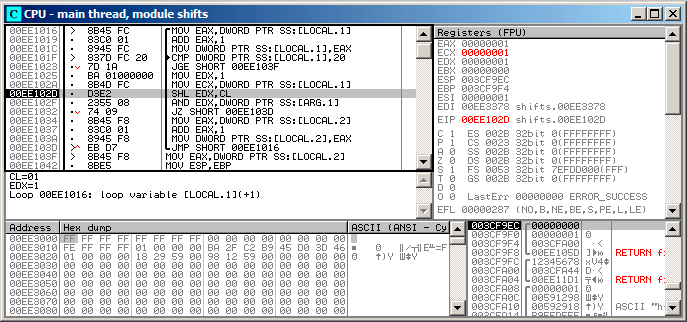
\includegraphics[scale=\FigScale]{patterns/14_bitfields/4_popcnt/olly1_1.png}
\caption{\olly: $i=1$, $i$ \RU{загружено в}\EN{is loaded into} \ECX}
\label{fig:shifts_olly1_1}
\end{figure}

\EDX \RU{содержит}\EN{is} $1$. \RU{Сейчас будет исполнена }\TT{SHL}\EN{ is to be executed now}.

\clearpage
\TT{SHL} \RU{исполнилась}\EN{was executed}:

\begin{figure}[H]
\centering
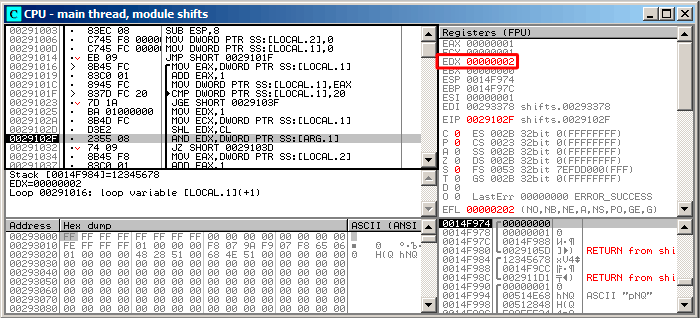
\includegraphics[scale=\FigScale]{patterns/14_bitfields/4_popcnt/olly1_2.png}
\caption{\olly: $i=1$, \EDX=$1 \ll 1=2$}
\label{fig:shifts_olly1_2}
\end{figure}

\EDX \RU{содержит}\EN{contain} $1 \ll 1$ (\OrENRU $2$). \RU{Это битовая маска}\EN{This is a bit mask}.

\clearpage
\ANDIns \RU{устанавливает}\EN{sets} \ZF \RU{в}\EN{to} $1$, 
\RU{что означает, что входное значение}\EN{which is meaning that input value} (\TT{0x12345678}) 
\RU{умножается\footnote{Логическое ``И''} с}\EN{ ANDed with} $2$ \RU{давая в результате}\EN{resulting} $0$:

\begin{figure}[H]
\centering
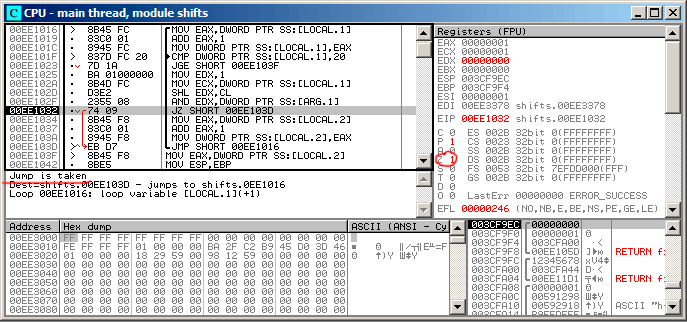
\includegraphics[scale=\FigScale]{patterns/14_bitfields/4_popcnt/olly1_3.png}
\caption{\olly: $i=1$, \RU{есть ли этот бит во входном значении? Нет.}
\EN{are there that bit in the input value? No.} (\ZF=1)}
\label{fig:shifts_olly1_3}
\end{figure}

\RU{Так что, во входном значении соответствующего бита нет}\EN{So, there are no corresponding bit in input value}.
\RU{Участок кода, увеличивающий счетчик бит на единицу не будет исполнен: инструкция \JZ \textit{обойдет} его}
\EN{The piece of code, which \glslink{increment}{increments} counter will not be executed: 
\JZ instruction will \textit{bypass} it}.

\clearpage
\RU{Я немного потрассировал далее и}\EN{Now I traced some time further and} $i$ \RU{теперь}\EN{is now} $4$.
\TT{SHL} \RU{исполнилась}\EN{is to be executed now}:

\begin{figure}[H]
\centering
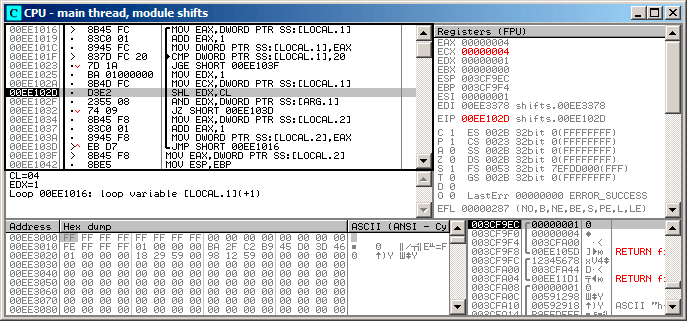
\includegraphics[scale=\FigScale]{patterns/14_bitfields/4_popcnt/olly4_1.png}
\caption{\olly: $i=4$, $i$ \RU{загружено в}\EN{is loaded into} \ECX}
\label{fig:shifts_olly4_1}
\end{figure}

\clearpage
\EDX=$1 \ll 4$ (\OrENRU \TT{0x10} \OrENRU $16$): 

\begin{figure}[H]
\centering
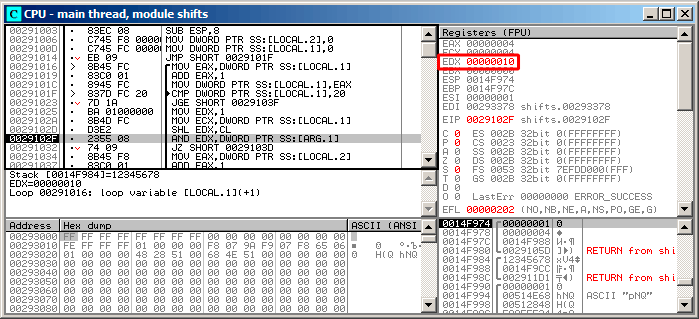
\includegraphics[scale=\FigScale]{patterns/14_bitfields/4_popcnt/olly4_2.png}
\caption{\olly: $i=4$, \EDX=$1 \ll 4=0x10$}
\label{fig:shifts_olly4_2}
\end{figure}

\RU{Это еще одна битовая маска}\EN{This is another bit mask}.

\clearpage
\ANDIns \RU{исполнилась}\EN{is executed}:

\begin{figure}[H]
\centering
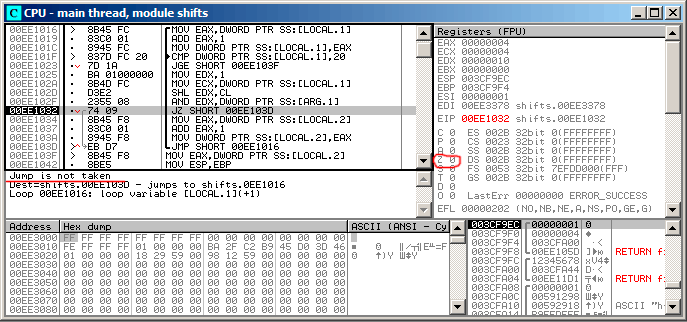
\includegraphics[scale=\FigScale]{patterns/14_bitfields/4_popcnt/olly4_3.png}
\caption{\olly: $i=4$, \RU{есть ли этот бит во входном значении? Да.}
\EN{are there that bit in the input value? Yes.} (\ZF=0)}
\label{fig:shifts_olly4_3}
\end{figure}

\ZF \RU{сейчас}\EN{is} $0$ \RU{потому что этот бит присутствует во входном значении}
\EN{because this bit is present in input value}.
\RU{Действительно}\EN{Indeed}, \TT{0x12345678 \& 0x10 = 0x10}. 
\RU{Этот бит считается: переход не сработает и счетчик бит будет увеличен на единицу}\EN{This bit counts: 
jump will not trigger and bits counter will be \glslink{increment}{incremented} now}.\\
\\
\RU{Ф-ция возвращает}\EN{The function returns} $13$. 
\RU{Это количество установленных бит в значении}\EN{This is total bits set in} \TT{0x12345678}\EN{ value}.


\subsubsection{GCC}

\RU{Скомпилируем то же и в}\EN{Let's compile it in} GCC 4.4.1:

\lstinputlisting[caption=GCC 4.4.1]{patterns/14_bitfields/4_popcnt/shifts_gcc.asm}

\subsection{x64}
\label{subsec:popcnt}

\RU{Я немного изменли пример, расширив его до 64-х бит}\EN{I modified the example slightly to extend it to 64-bit}:

\lstinputlisting[label=popcnt_x64_example]{patterns/14_bitfields/4_popcnt/shifts64.c}

\subsubsection{\NonOptimizing GCC 4.8.2}

\RU{Пока всё просто}\EN{So far so easy}.

\lstinputlisting[caption=\NonOptimizing GCC 4.8.2]{patterns/14_bitfields/4_popcnt/shifts64_GCC_O0.s.\LANG}

\subsubsection{\Optimizing GCC 4.8.2}

\lstinputlisting[caption=\Optimizing GCC 4.8.2,numbers=left,label=shifts64_GCC_O3]{patterns/14_bitfields/4_popcnt/shifts64_GCC_O3.s.\LANG}

\RU{Код более лаконичный, но содержит одну необычную вещь}\EN{This code is terser, but has a quirk}.
\RU{Во всех примерах, что мы пока видели, инкремент значения переменной ``rt'' происходит после сравнения 
определенного бита с единицей, но здесь ``rt'' увеличивается на 1 до этого (строка 6), записывая новое значение
в регистр \EDX.}
\EN{In all examples that we see so far, we were incrementing the ``rt'' value after comparing a specific bit,
but the code here increments ``rt'' before (line 6), writing the new value into register \EDX .}
\RU{Затем, если последний бит был 1, инструкция}\EN{Thus, if the last bit is 1, the} \TT{CMOVNE}
\footnote{Conditional MOVe if Not Equal\RU{ (MOV если не равно)}}\EN{ instruction} 
(\RU{которая синонимична}\EN{which is a synonym for} \TT{CMOVNZ}
\footnote{Conditional MOVe if Not Zero\RU{ (MOV если не ноль)}}) \IT{\RU{фиксирует}\EN{commits}} 
\RU{новое значение}\EN{the new value of} ``rt''
\RU{копируя значение из}\EN{by moving} \EDX (``\RU{предполагаемое значение rt}\EN{proposed rt value}'') 
\RU{в}\EN{into} \EAX 
(``\RU{текущее}\EN{current} rt'' \RU{которое будет возвращено в конце ф-ции}\EN{to be returned at the end}).
\RU{Следовательно, инкремент происходит на каждом шаге цикла, т.е., 64 раза, вне всякой связи с входным
значением.}
\EN{Hence, the incrementing is done at each step of loop, i.e., 64 times, without any relation to the input value.}

\RU{Преимущество этого кода в том, что он содержит только один условный переход (в конце цикла) вместо
двух (пропускающий инкремент ``rt'' и еще один в конце цикла).}
\EN{The advantage of this code is that it contain only one conditional jump (at the end of the loop) instead of 
two jumps (skipping the ``rt'' value increment and at the end of loop).}
\RU{И это может работать быстрее на современных CPU с предсказателем переходов}
\EN{And that might work faster on the modern CPUs with branch predictors}: \ref{branch_predictors}.

\label{FATRET}
\index{x86!\Instructions!FATRET}
\RU{Последняя инструкция это}\EN{The last instruction is} \TT{REP RET} (\EN{opcode}\RU{опкод} \TT{F3 C3}) 
\RU{которая также называется}\EN{which is also called} \TT{FATRET} \RU{в}\EN{by} MSVC.
\RU{Это оптимизированная версия \RET, рекомендуемая AMD для вставки в конце ф-ции, если \RET идет
прямо после условного перехода}\EN{This is somewhat optimized version of \RET, 
which is recommended by AMD to be placed at the end of function, if \RET goes right after conditional jump}: 
\cite[p.15]{AMDOptimization}
\footnote{\RU{Больше об этом}\EN{More information on it}: \url{http://go.yurichev.com/17328}}.

\subsubsection{\Optimizing MSVC 2010}

\lstinputlisting[caption=MSVC 2010]{patterns/14_bitfields/4_popcnt/MSVC_2010_x64_Ox.asm.\LANG}

\index{x86!\Instructions!ROL}
\RU{Здесь используется инструкция}\EN{Here the} \TT{ROL} \RU{вместо}\EN{instruction is used instead of} 
\TT{SHL}, \RU{которая на самом деле}\EN{which is in fact} ``rotate left''\RU{ (прокручивать влево)} 
\RU{вместо}\EN{instead of} ``shift left''\RU{ (сдвиг влево)},
\RU{но здесь, в этом примере, она работает так же как и}\EN{but in this example 
it will work just as} \TT{SHL}.

\RU{Об этих ``прокручивающих'' инструкциях больше читайте здесь}\EN{You can read more about the rotate instruction 
here}: \ref{ROL_ROR}.

\Reg{8} \RU{здесь считает от 64 до 0}\EN{here is counting from 64 to 0}. 
\RU{Это как бы инвертированная переменная $i$}\EN{It's just like an inverted $i$}.

\RU{Вот таблица некоторых регистров в процессе исполнения}\EN{Here is a table of some registers during the execution}:

\begin{center}
\begin{tabular}{ | l | l | }
\hline
\cellcolor{blue!25} RDX & \cellcolor{blue!25} R8 \\
\hline
0x0000000000000001 & 64 \\
\hline
0x0000000000000002 & 63 \\
\hline
0x0000000000000004 & 62 \\
\hline
0x0000000000000008 & 61 \\
\hline
... & ... \\
\hline
0x4000000000000000 & 2 \\
\hline
0x8000000000000000 & 1 \\
\hline
\end{tabular}
\end{center}

\index{x86!\Instructions!FATRET}
\RU{В конце видим инструкцию}\EN{At the end we see the} \TT{FATRET}\RU{, которая была описана здесь}\EN{ instruction, 
which was explained here}: \ref{FATRET}.

\subsubsection{\Optimizing MSVC 2012}

\lstinputlisting[caption=MSVC 2012]{patterns/14_bitfields/4_popcnt/MSVC_2012_x64_Ox.asm.\LANG}

\index{\CompilerAnomaly}
\label{MSVC2012_anomaly}
\Optimizing MSVC 2012 \RU{делает почти то же самое что и оптимизирующий}\EN{does almost the same job as 
optimizing} MSVC 2010, \RU{но почему-то, он генерирует 2 идентичных тела цикла и счетчик цикла теперь 32
вместо 64}\EN{but somehow, it generates two identical loop bodies and the loop count is now 32 instead of 64}.
\RU{Честно говоря, я не знаю, почему. Какой-то трюк с оптимизацией? Может быть, телу цикла лучше быть
немного длиннее?}
\EN{To be honest, I don't know why. Some optimization trick? Maybe it's better for the loop body to be slightly 
longer?}
\RU{Так или иначе, я сознательно добавляю такой код здесь чтобы показать, что результат компилятора
иногда может быть очень странный и нелогичный, но прекрасно работающий, конечно же.}
\EN{Anyway, I have added the code here intentionally to show that sometimes the compiler output may be really weird and 
illogical, but perfectly working.}

\ifdefined\IncludeARM
\subsection{ARM + \OptimizingXcodeIV (\ARMMode)}

\lstinputlisting[caption=\OptimizingXcodeIV (\ARMMode),label=ARM_leaf_example4]{patterns/14_bitfields/4_popcnt/ARM_Xcode_O3.lst.\LANG}

\index{ARM!\Instructions!TST}
\TT{TST} \RU{это то же что и}\EN{is the same things as} \TEST \InENRU x86.

\index{ARM!Optional operators!LSL}
\index{ARM!Optional operators!LSR}
\index{ARM!Optional operators!ASR}
\index{ARM!Optional operators!ROR}
\index{ARM!Optional operators!RRX}
\index{ARM!\Instructions!MOV}
\index{ARM!\Instructions!TST}
\index{ARM!\Instructions!CMP}
\index{ARM!\Instructions!ADD}
\index{ARM!\Instructions!SUB}
\index{ARM!\Instructions!RSB}
\RU{Как я уже указывал}\EN{As I mentioned before}~(\myref{shifts_in_ARM_mode}),
\RU{в режиме ARM нет отдельной инструкции для сдвигов.}
\EN{there are no separate shifting instructions in ARM mode.}
\RU{Однако, модификаторами}\EN{However, there are modifiers} 
LSL (\IT{Logical Shift Left}), 
LSR (\IT{Logical Shift Right}), 
ASR (\IT{Arithmetic Shift Right}), 
ROR (\IT{Rotate Right}) \AndENRU 
RRX (\IT{Rotate Right with Extend}) \RU{можно дополнять некоторые инструкции, такие как}
\EN{, which may be added to such instructions as} \MOV, \TT{TST},
\CMP, \ADD, \SUB, \TT{RSB}\footnote{\DataProcessingInstructionsFootNote}.

\RU{Эти модификаторы указывают, как сдвигать второй операнд, и на сколько.}
\EN{These modificators define how to shift the second operand and by how many bits.}

\index{ARM!\Instructions!TST}
\index{ARM!Optional operators!LSL}
\RU{Таким образом, инструкция }\EN{Thus the} \TT{``TST R1, R2,LSL R3''} 
\RU{здесь работает как}\EN{instruction works here as} $R1 \land (R2 \ll R3)$.

\subsection{ARM + \OptimizingXcodeIV (\ThumbTwoMode)}

\index{ARM!\Instructions!LSL.W}
\index{ARM!\Instructions!LSL}
\RU{Почти такое же}\EN{Almost the same}, 
\RU{только здесь применяется пара инструкций}\EN{but here are two} 
\TT{LSL.W}/\TT{TST} 
\RU{вместо одной}\EN{instructions are used instead of a single} 
\TT{TST},
\RU{ведь в режиме thumb нельзя добавлять указывать модификатор}\EN{because in thumb mode it is not
possible to define} \TT{LSL} \RU{прямо в}\EN{modifier directly in} \TT{TST}.

\begin{lstlisting}[label=ARM_leaf_example5]
                MOV             R1, R0
                MOVS            R0, #0
                MOV.W           R9, #1
                MOVS            R3, #0
loc_2F7A
                LSL.W           R2, R9, R3
                TST             R2, R1
                ADD.W           R3, R3, #1
                IT NE
                ADDNE           R0, #1
                CMP             R3, #32
                BNE             loc_2F7A
                BX              LR
\end{lstlisting}

\subsection{ARM64 + \Optimizing GCC 4.9}

\RU{Я взял 64-битный пример, который уже использовал}\EN{I took the 64-bit example I already used}: 
\myref{popcnt_x64_example}.

\lstinputlisting[caption=\Optimizing GCC (Linaro) 4.8]{patterns/14_bitfields/4_popcnt/ARM64_GCC_O3.s.\LANG}

\RU{Результат очень похож на тот, что GCC сгенерировал для x64}\EN{The result is very similar to what GCC 
generates for x64}: \myref{shifts64_GCC_O3}.

\index{ARM!\Instructions!CSEL}
\EN{The}\RU{Инструкция} \TT{CSEL} \RU{это}\EN{instruction is} ``Conditional SELect''\RU{ (выбор при условии)}, 
\RU{она просто выбирает одну из переменных, в зависимости от флагов выставленных}\EN{it just choose one 
variable of two depending on the flags set by} \TT{TST} \RU{и копирует значение в регистр}\EN{and copies the value 
into} \RegW{2}\RU{, содержащий переменную ``rt''}\EN{ , which holds the ``rt'' variable}.

\subsection{ARM64 + \NonOptimizing GCC 4.9}

\RU{И снова, я использовал 64-битный пример, который я уже использовал раннее}\EN{And again, the 64-bit 
example I already used}: \myref{popcnt_x64_example}.

\RU{Код более многословный, как обычно}\EN{The code is more verbose, as usual}.

\lstinputlisting[caption=\NonOptimizing GCC (Linaro) 4.8]{patterns/14_bitfields/4_popcnt/ARM64_GCC_O0.s.\LANG}

\fi
\ifdefined\IncludeMIPS
\subsection{MIPS}

\subsubsection{\NonOptimizing GCC}

\lstinputlisting[caption=\NonOptimizing GCC 4.4.5 (IDA)]{patterns/14_bitfields/4_popcnt/MIPS_O0_IDA.lst.\LANG}

\index{MIPS!\Instructions!SLL}
\index{MIPS!\Instructions!SLLV}
\RU{Это многословно: все локальные переменные расположены в локальном стеке и перезагружаются каждый раз,
когда нужны.}
\EN{That is verbose: all local variables are located in the local stack and reloaded each time they're needed.}
\RU{Инструкция SLLV это \q{Shift Word Left Logical Variable}, она отличается от SLL только тем что
количество бит для сдвига кодируется в SLL (и, следовательно, фиксировано), а SLL берет количество из регистра.}
\EN{The SLLV instruction is \q{Shift Word Left Logical Variable}, it differs from SLL only in that
the shift amount is encoded in the SLL instruction (and is fixed, as a consequence), 
but SLLV takes shift amount from a register.}

\subsubsection{\Optimizing GCC}

\RU{Это более сжато}\EN{That is terser}.
\RU{Здесь две инструкции сдвигов вместо одной.}\EN{There are two shift instructions instead of one.}
\RU{Почему}\EN{Why}?
\RU{Можно заменить первую инструкцию SLLV на инструкцию безусловного перехода, передав управление прямо
на вторую SLLV.}
\EN{It's possible to replace the first SLLV instruction with an unconditional branch instruction that 
jumps right to the second SLLV.}
\RU{Но это еще одна инструкция перехода в функции, а от них избавляться всегда выгодно}
\EN{But this is another branching instruction in the function, and it's always favorable to get rid of them}: 
\myref{branch_predictors}.

\lstinputlisting[caption=\Optimizing GCC 4.4.5 (IDA)]{patterns/14_bitfields/4_popcnt/MIPS_O3_IDA.lst.\LANG}

\fi
